\documentclass{article}
\usepackage[margin=1.0in]{geometry}
\usepackage{listings}
\usepackage{xcolor}
\usepackage{graphicx}
\usepackage{siunitx}
\usepackage{float}
\usepackage{setspace}
\usepackage{makecell}
\usepackage{gensymb}
\usepackage{url}
\usepackage{placeins}
\usepackage{caption}
\usepackage{inconsolata}
\usepackage{booktabs}
\usepackage{hyperref}
\usepackage{float} % Add this in your preamble

\title{ELEC 291 : Metal Detecting Robot}
\author{Team A9}
\date{April 12th, 2024}

\definecolor{codegreen}{rgb}{0,0.6,0}
\definecolor{codegray}{rgb}{0.5,0.5,0.5}
\definecolor{codepurple}{rgb}{0.58,0,0.82}
\definecolor{backcolour}{rgb}{0.95,0.95,0.92}

\lstdefinestyle{mystyle}{
    backgroundcolor=\color{backcolour},
    commentstyle=\color{codegreen},
    keywordstyle=\color{magenta},
    numberstyle=\tiny\color{codegray},
    stringstyle=\color{codepurple},
    basicstyle=\footnotesize\ttfamily,
    breakatwhitespace=false,
    breaklines=true,
    captionpos=b,
    keepspaces=true,
    numbers=left,
    numbersep=5pt,
    showspaces=false,
    showstringspaces=false,
    showtabs=false,
    tabsize=2
}

\linespread{1.6}
\setlength{\parindent}{0pt} % Disable paragraph indentation

\lstset{style=mystyle}

\begin{document}

\maketitle
\begin{center}
Course: ELEC 291/292 Electrical Engineering Design Studio I \\
Section: L2A \\
Instructor: Dr. Jesus Calvino-Fraga \\
\end{center}

\begin{center}
\begin{tabular}{|c|c|c|c|}
    \hline
    Student \# & Student Name & \%Points & Signature \\
    \hline
    67286750 & Tomaz Zlindra & 120 & 
\includegraphics[width = 1.5cm]{Names/Tomaz.jpeg}  \\
    \hline
    21475330 & Martin Lieu & 100 &
    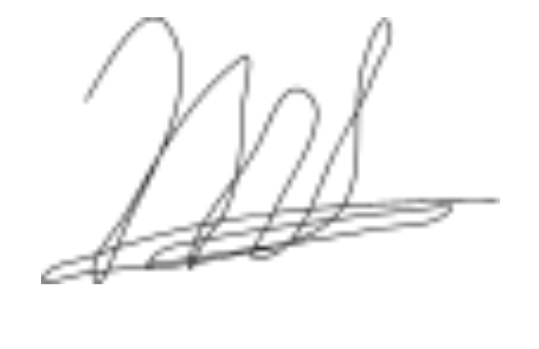
\includegraphics[width=1.5cm]{Names/Martin.png} \\
    \hline
    7106221 & Muntakim Rahman & 120 & 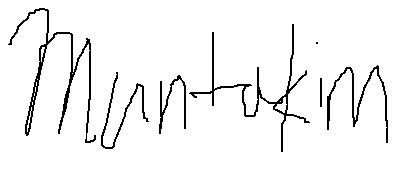
\includegraphics[width=1.5cm]{Names/Muntakim.png} \\
    \hline
    76029933 & James Huang & 60 & 
\includegraphics[width = 1.5cm]{Names/James.jpeg}\\
    \hline
    17542499 & Emile Jansen  & 95 & 
\includegraphics[width = 1.5cm]{Names/Emile.png} \\
    \hline
    46634911 & Kyden McCaskill & 105 & 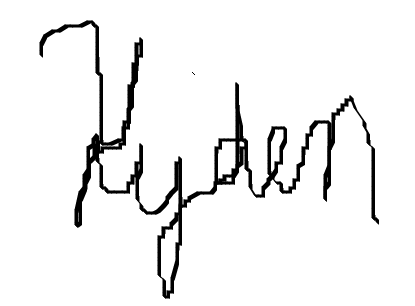
\includegraphics[width=1.5cm]{Names/Kyden.png}\\
    \hline
\end{tabular}
\end{center}

\newpage

\tableofcontents

\newpage
\section{Introduction}

\subsection{Objective}

The purpose of this project was to develop a metal detecting robot. The robot was required to be
battery operated and wirelessly controlled with a joystick. The controller is used enable smooth control of the robot's
motors, determining its direction and speed. It should also notify the user when the robot detects metal, via an LCD
display and speaker. It should be able to differentiate between the metals detected by inductance, as well as sound.

\

The ultimate goal of the project was to apply the learnings from the second set of labs in this course, with two separate families of microcontrollers.
The circuitry used was familiar to prior labs in this course, but is designed to enable firmware detection of inductance with electromagnetism theory.

\subsection{System Block Diagrams}

In order to meet these system requirements and specifications, we designed the hardware and software as shown in the system diagrams below.
We will refer to these later in the report.

\begin{figure}[h]
    \centering
    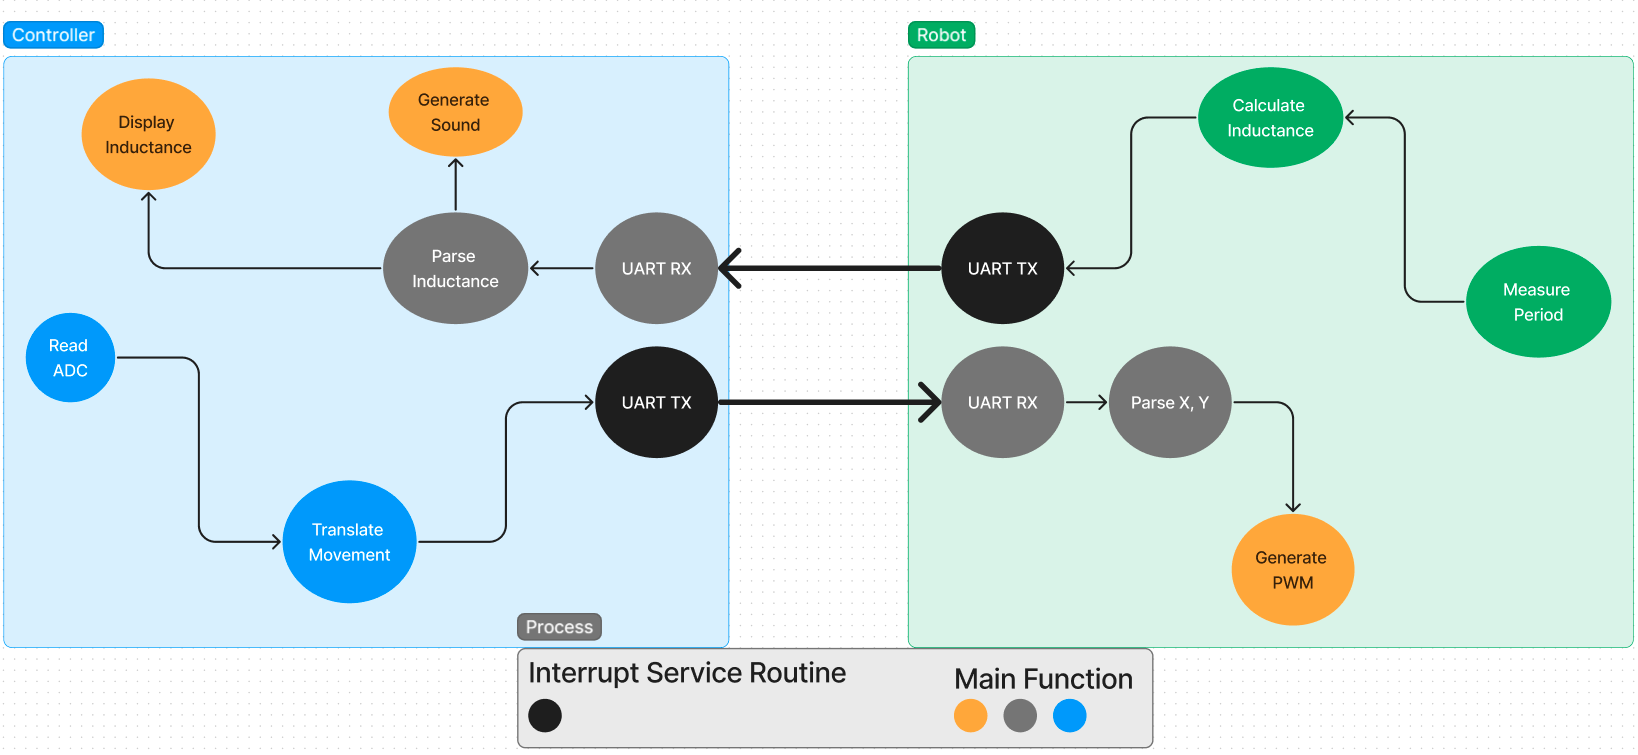
\includegraphics[width=1\linewidth]{Figures/Firmware_Block_Diagram.png}
    \caption{Firmware Block Diagram}
    \label{fig:firmware_block_diagram}
\end{figure}

\section{Investigation}

Prior to settling on a final design, we individually and collaboratively scoped out the
constraints of our project components (listed in the project requirements in Table \ref{table:project_requirements}).

\subsection{Idea Generation}

We generated ideas for the robot implementation by discussing the process for meeting a set of predetermined specifications.
This allowed us to dissect the problem into smaller and more manageable parts, as well as effective task allocation for firmware and
hardware development. We discussed how each of these parts would work together to yield a fully functional robot. We prototyped individual components
in isolated test environments to confirm details, such as the functionality of the joystick and PWM peripherals, the performance of the movement logic,
and the JDY-40 transmission between microcontrollers. Integrating these functional components into a functional product was the
final step, allowing us to fine-tune initial designs collaboratively through end-to-end testing.

\subsection{Investigation Design}

To begin our design, we leveraged our knowledge of Labs 4-6 to understand how circuitry and software modules should be implemented.
A few components required further research, such as the Colpitts Oscillator for the metal detector, and the JDY-40 radio module for data transmission. %ToDo : Add Bibliography
For our circuitry, we referred to datasheets to ensure our electrical components were powered in the appropriate voltage ranges.
We also determined capacitances which would enable a stable steady state for the Colpitts Oscillator and for us to meet expected inductance values.
We spent some time understanding the limitations of the JDY-40 and how to properly configure them for communication between the two microcontrollers.

\subsection{Data Collection}

We collected data through extensive user testing, both individually and as a group. This was akin to regression testing in software development.
The key process consisted of using the controller to move the robot and ensuring it met expectations. We debugged the JDY-40 communication with
\texttt{printf(tx\_data);} and \texttt{printf(rx\_data);} statements, as well as ensuring the system predictably responded to the provided inputs.

\

Qualitative testing involved trying to smoothly maneuver the robot in the desired paths (i.e. straight line, square formation, figure-8 formation, etc.), as well as
the ability to indicate metal objects which were detected (i.e. via LCD display and speaker).

\

To quantitatively measure performance, the lab equipment (i.e. oscilloscope, multimeter) was used to measure the signals and ensure they were within
the expected range. This was especially useful in timing our Interrupt Service Routines (ISRs) and ensuring that the PWM signals were generated correctly.
To test non-PWM timers, we toggled microcontroller pins to ensure the ISRs were being executed at the correct frequency.

\subsection{Data Synthesis}

During testing, we emphasized having peer group members evaluate the performance of individual modules (i.e. movement controls, inductance detection, JDY-40 communication) to
ensure that the system was functioning as expected. The lead developer of the given module participated in Quality Assurance (QA) testing as well, but needed feedback from others to
ensure we were able to address bugs without bias. This was especially useful in evaluating JDY-40 communication for the movement controls and inductance detection.

\

We also developed a Python script to access the microcontroller COM ports and log both the movement and inductance data shared between the microcontrollers. This enabled validation of
response time and accuracy betweeen transmitted and received data streams.

\begin{figure}[htbp]
    \centering
    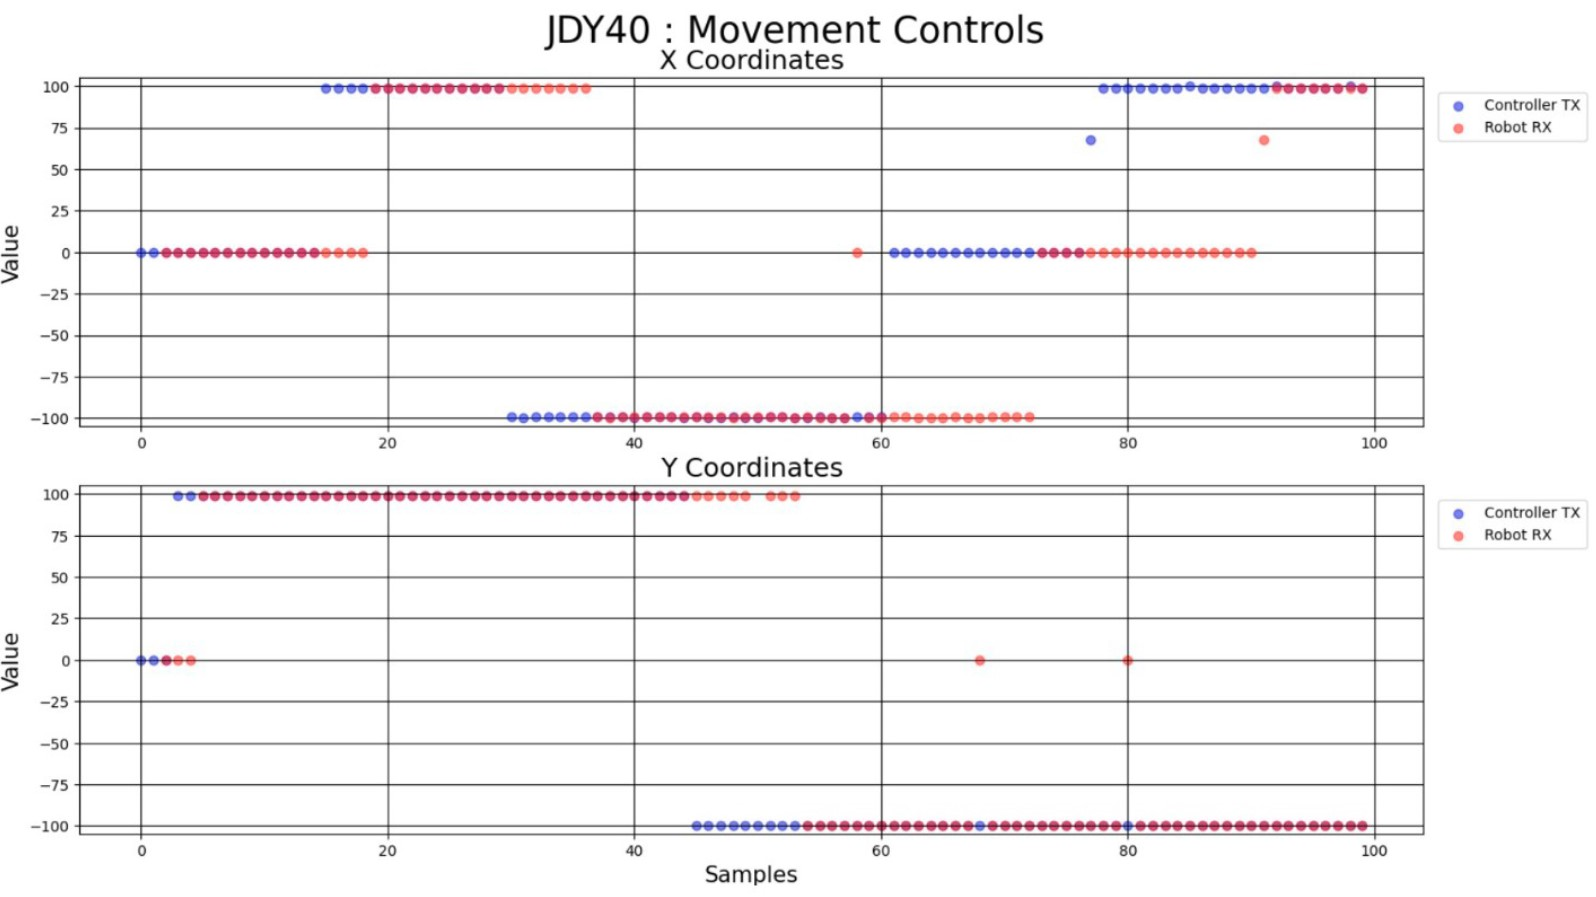
\includegraphics[width=1\textwidth]{Figures/Movement_Logs.jpg}
    \caption{Movement Controls : Data Logs}
    \label{fig:movement_controls_logs}
\end{figure}

\begin{figure}[htbp]
    \centering
    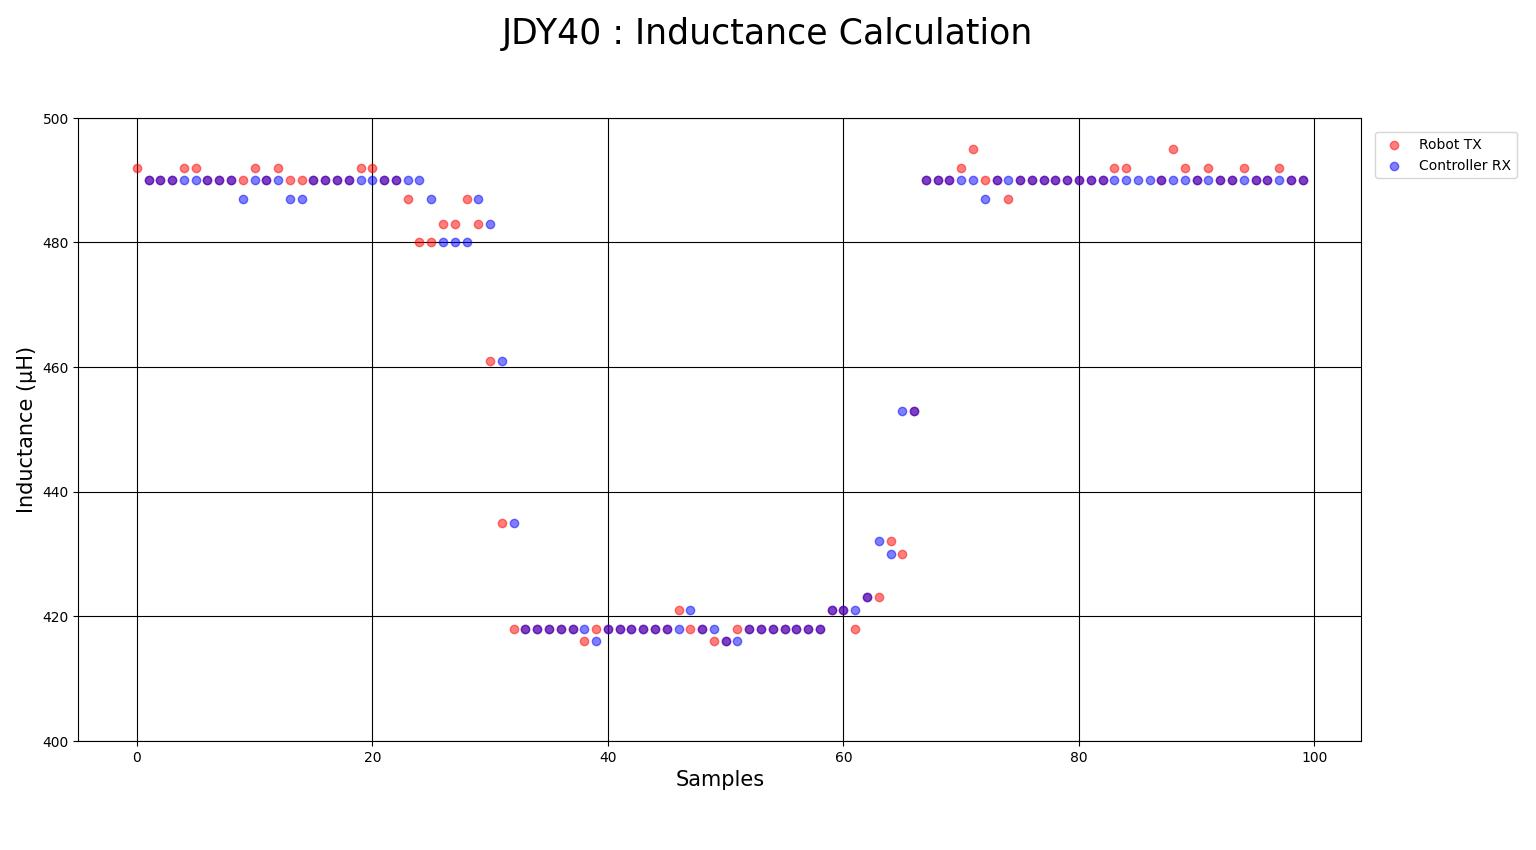
\includegraphics[width=1\textwidth]{Figures/Inductance_Logs.jpg}
    \caption{Inductance Detection : Data Logs}
    \label{fig:inductance_detection_logs}
\end{figure}

\subsection{Analysis of Results}

From the graphs in Figures \ref{fig:movement_controls_logs} and \ref{fig:inductance_detection_logs}, we noted that the latency is displayed as a number of samples. This was due to the fact that we had
many samples per second and wanted to visualize the microcontroller responsiveness to new information. In Figure \ref{fig:movement_controls_logs}, we
see that the direction and speed was transmitted accurately from the STM32 to the EFM8. We modified both X and Y coordinates to test possible combinations and this was received in a reasonable number of samples.
In Figure \ref{fig:inductance_detection_logs}, we see that the inductance values exhibited similar transmission behavior upon change.

\

The inductance experienced latency issues early on in the development process and we underwent many iterations on our
firmware implementation to ensure that the period was measured accurately and we were able to calculate an inductance which could be
used to determine magnetic thresholds. Note that it was important to be able to bucketize inductance ranges
(i.e. 400-500 mH, 500-600 mH, etc) to determine variations in metal detected.

\section{Design}

As we settled on preliminary designs of our subsystems, we required approval from team members to ensure requirements and constraints
were addressed in our thought processes.

\subsection{Use of Process}

We followed the Work Breakdown Structure (WBS) principle during development. A well planned design of individual elements ensured that we could
develop and test each module independently. This allowed us to identify and address issues in the early stages of development, hence
effectively combine building blocks.

\

Another process we emphasized was keeping track of software revisions in a well managed Git repository. We used Visual Studio Code: Live Share
to collaborate on the same codebase and to ensure that we were able to debug and test the code in real-time.

\

This was especially useful during dedicated group work sessions where we were adding adjacent features to a development branch.
We pushed the local branch to the remote repository (for access and transparency), and merged it with the main branch after ensuring it works
exactly as intended on the microcontrollers. Tracking firmware revisions with source control also enabled quick iterations on software modules,
which helped us meet project timelines.

\

Requirement functionality was prioritized in the integration process, including the movement controls, inductance detection, and JDY-40 communication.
The additional features (i.e. lock/unlock, speed limiter, turn limiter) were added after the core functionality was confirmed to be working as expected. This was due to an emphasis
on meeting the project objective.

\subsection{Need and Constraint Identification}
During firmware development, we identified the following constraints from the
documents provided by Dr. Jesus Calvino-Fraga \cite{RequirementsPDF}, as well as from our own comprehension:

\begin{table}[ht]
    \center
    \begin{tabular}{|l|p{0.6\linewidth}|}
        \hline
        \textbf{Requirements} \\ \hline
        The controller and robot must be driven by two microcontrollers from \\
        different families (e.g., ARM Cortex and 8051). \\ \hline
        The robot must be able to detect metal using an inductor built from \\
        magnet wire and a coil frame. \\ \hline
        The robot must be powered by AA batteries to drive wheels and 9V for \\
        the remaining functions. \\ \hline
        The speed and direction of the robot must be smoothly controlled with a joystick. \\ \hline
        The controller and the robot must wirelessly transmit data to one another. \\ \hline
        The metal detected by the robot should be indicated to \\
        the user via visual and auditory feedback. \\ \hline
        The transmission of data must be reliable and accurate. \\ \hline
    \end{tabular}
    \caption{List of Project Requirements}
    \label{table:project_requirements}
\end{table}

\subsection{Problem Specification}

We encountered several related and recurring issues throughout the project, including inaccurate period measurements of the
Colpitts Oscillator, unreliable JDY-40 communications between the microcontrollers, and
the overall code integration between modules.

\

\textbf{JDY-40 Communications} \\
A key module which required extensive development time was the JDY-40 communication between the STM32 and EFM8 microcontrollers.
The bugs caused by this were the main blocker in integrating our firmware, as the communication was not reliable and often failed to transmit
data between the two microcontrollers.

\

In our design, we decided to time the transmission of data to ensure transmission occurred at a consistent rate (i.e. via ISR).
This was to avoid the usage of synchronous delays, which block the execution of other code. We timed the ISR transmission to strike a balance,
ensuring it wasn't excessively slow or fast. Otherwise, we risked losing data due to transmitting too quickly or rendered it obsolete
due to slow data transmission. We also had to ensure that the data was sent in a format that could be easily and accurately parsed by the
receiving microcontroller.

\

We also had to ensure that the data was sent in a format that could be easily parsed by the receiving microcontroller. This was especially important in translating the
X and Y coordinates from the joystick to the robot microcontroller.

\

A major obstacle was finding that Git commits with a functional JDY-40 module would suddenly behave erratically
(i.e. transmission delays, inaccurate data to be received). We believe this was partially due to software bugs, but also due to the high number of JDY-40s in the lab environment during the latter part of the project.

\

\textbf{Period Measurement} \\
Although a seemingly trivial task, measuring a period which altered by less than
1ms was difficult to measure accurately. This was due to the implementation with EFM8 Timer 0,
which monitored the number of clock cycles for a period signal during $n$ periods.

\

By nature, this needed to be an uninterrupted calculation such that the period could be accurately measured. We found that the period was often inaccurate due to the ISRs we implemented for
parallel functionality (i.e. JDY-40 communication, PWM generation). To overcome this, we had to disable all other ISRs during the period calculation to ensure an accurate reading.

\

\textbf{Integration} \\
Integrating all the code together was a major obstacle, partially due to the issue mentioned above. We tested our firmware modules and observed functionality
individually, but when we combined them, we found that the code would often malfunction.

One example of this was when we added the JDY-40 program to the speaker code on the STM32. We had configured Timer 2 in PWM mode via Channel 1, which
required a pin in conflict with the UART2 peripheral. Another key example was when we incorporated the JDY-40 code with the PWM code
on the EFM8. Timer 3 was being used for a JDY-40 delay, but we also needed to use Timer 3 for the PWM generation. This required us to
reconfigure the PWM to use Timer 5 ISR to ensure that they were not in conflict with one another.

\subsection{Solution Generation}

We found that the best way to develop our solution was through the same four-step process adhered to in the Oven Reflow Controller in Project 1.
This involved :

\begin{enumerate}
  \item Discussing the individual requirements and assigning development to team members.
  \item Developing sub modules in a test environment.
  \item Integrating the sub modules into a single, cohesive product.
  \item Exhaustively test and debug functionality until requirements are met.
\end{enumerate}

To address recurring and ongoing issues, we relied on the WBS principle to isolate them from the rest of our system.
This was critical in investgating the firmware issues related to the JDY-40 radio and to understand whether the transmission rate was the culprit
in unreliable and inaccurate data. We also identified that the issue with period measurement could be solved by thwarting ISR execution during the period calculation.

\

Once we established functionality in these test environments, we were able to hone in on the root cause of issues, before developing solutions to address them. This was most evident
in our reconfiguration of timers to deal with conflicts in between modules (i.e. speaker and JDY-40 on the STM32, JDY-40 and PWM on the EFM8).

\

When redesigning the JDY-40 communication, we started from the test C program provided by Dr. Jesus Calvino-Fraga.

\

We incrementally added code to the core (albeit limited) functionality of this program to determine the cause behind
the erratic behavior. We initially had both the UART transmission and reception in ISRs for both microcontrollers, but we observed that receiving data asynchronously
caused our microcontroller to crash. We soon realized this functionality should be synchronous and a part of the main program.
Since the response to an input is a synchronous process, we should receive the input synchronously as well. However, we appreciated being able to
control the timing of transmission to ensure that the data was sent at a consistent rate. Due to this, we continued to use ISRs for transmission,
and these were the contributing factor in transmission rate.

\

Collaboratively tackling discovered problems allowed us to address them comprehensively and perform extensive testing during the
development process. We also found that ownership over individual subcomponents allowed us to effectively identify the problems in the section above. Having a group member
more familiar with a specific subsystem was critical in swiftly addressing development challenges.


\subsection{Solution Evaluation}

To evaluate our final implementation, we emphasized end-to-end testing. This involved adding modules incrementally and seeing how they interact with one another to
perform intended functions. Stress testing the controls was a key part of this, as we wanted to ensure that the robot could move the way the user intends. Since the user is not necessarily someone who
requires context to our engineered solution, we included group members working on adjacent functionality to test and evaluate our solutions. If the robot met a qualitative checklist
of adequate response time, accuracy, and reliability (as determined by the user), we considered the implementation successful. This was especially important once we had quantiatively tracked the
output of signals with the lab equipment and with \texttt{printf();} statements. Since the modules functioned by themselves in a test environment, and functioned together as observed with
available tools, user testing was our final and conclusive evaluation metric.

\subsection{Safety/Professionalism}

To ensure our product was safe, we developed many safety algorithms in the program. Before the robot could be controlled, the user had to enter a 4 digit passcode
to "unlock" the remote controller. This was paired with a lock feature which would disable the controller in the need of an emergency or other purpose. In tandem with this,
we had a power switch to both conserve battery life and to ensure that the robot could not be controlled in this state. In addition, we implemented a speed limiter and turn
limiter on the remote controller for the movement of the robot. If the user wished to operate at a lower speed without the risk of too much speed, a simple click would enable this.

\

Furthermore, all this information was displayed on an LCD to provide visual feedback of the controller settings.
To ensure professionalism, we maintained a clean and organized codebase, and managed development updates with good source control practices. We also maintained a professional
attitude in our communication and collaboration during the project.

\subsection{Detailed Design}

\subsubsection{Hardware Design}
The robot's EFM8 circuit and the controller's STM32 circuit were intricate systems, featuring numerous connections. However, these were not complex in design.

\

As seen in the Figure \ref{fig:stm32} (STM32 Hardware Diagram), the relevant circuits include the voltage dividers, joystick (ADC), JDY-40, and LCD. Conversely, in the Figure \ref{fig:efm8} (EFM8 Hardware Diagram), the important circuits
were the voltage dividers, JDY-40, metal detector and optocoupler/H-bridge circuits.

\

\textbf{Voltage Dividers} \\
We had a total of 4 step down voltage dividers for this project. Since the controller and the robot needed to be battery powered, we were required to use an LM7805 to drop the voltage of a standard 9V alkaline battery to 5V to power circuits such as the EFM8, LCD, speakers and the metal detector circuit. For stabilizing capacitors we used 0.22$\mu$F and 0.1$\mu$F capacitors as shown in the LM7805 datasheet\cite{LM7805}. Subsequently, this 5V voltage was also dropped down to a voltage of 3v3 using the MCP-1700 to power the ADC, JDY-40s and the STM32. We used 2 1$\mu$F capacitors to stabilize the signal (as suggested in the datasheet\cite{MCP1700}).

\

\textbf{ADC Joystick} \\
The PS2 joystick was a basic dual ADC device to control the robot. This also did not require any complex designs as it is just two potentiometers in the x and y directions. This device was connected to 3V3 with the VRX and VRY pins connected to two ADC pins on the STM32 to measure ADC values. We also ended up using the built-in switch as a seperate button connected to a GPIO pin on the microcontroller.

\

\textbf{JDY-40 Circuit} \\
The JDY-40 (\ref{fig:JDY-40}) was used on both controller and the robot for wireless communication. The wiring was very straightforward, it was powered with 3V3 and the TX and RX pins are connected to the RX and TX pins, respectively. The SET pin was connected to a basic GPIO output on the microcontroller, used during the pairing process for AT commands (set to GND whenever an AT command needed to be sent).

\

\textbf{Metal Detector Circuit} \\
To detect metal, we used Colpitts Oscillator (\ref{fig:metaldetector}) with a discrete CMOS Inverter. This would allow us to measure a frequency related to the inductance of the inductor by using the formula $f = \frac{1}{2 \pi \sqrt{LC_T}}$, where $C_T = \frac{C_1C_2}{C_1+C_2}$. Since we wanted to use lower capacitances to allow for a larger $\Delta f$, we ended up using $C_1 =$ 1nF and $C_2 =$ 10nF. This allowed for a stable steady state and were also within the recommended range proposed by Dr. Jesus Calvino-Fraga \cite{SlidesPDF}.

\

% optocoupler and H-bridge section
\textbf{Optocoupler and H-Bridges} \\
In order to convert our voltage PWM signal into a movable operation, we needed the h-bridge and optocouplers for each motor. The H-bridges would switch the polarity of the applied voltage, enabling for forward or backwards motion depending on the strength of the applied signal. Furthermore, the contrasting high voltage operations of the motor and low voltage operations from the EMF8 is an electrical concern that we addressed by implementing the optocouplers. The optocouplers electrically isolate the two circuits, preventing voltage spikes and limiting noise, improving compatibility and efficiency. \\
Additionally, we used adequate resistors values to satisfy the 50\% current transfer ratio (CTR) and other conditions to achieve proper functionality\cite{LTV-847}.

\subsubsection{Firmware Design}
This project required a strong firmware foundation to ensure the robot behaved as intended. This entailed developing $C$ programs in close coordination for the STM32 and EFM8 systems.
The fundamental modules include the joystick input standardization, movement logic/PWM control, JDY-40 communications, speakers, period calculations (metal detector) and a passcode menu on the controller.

\

\textbf{Joystick Input Standardization} \\
The raw ADC values from the joystick were not sent directly to the robot microcontroller. First, we subtracted the values by the initial ADC values they had initially (around $\frac{2^{12}-1}{2}$), to ensure when the joystick is in the middle, the value was 0.

\begin{lstlisting} [language=C, caption={Joystick Calibration}, label={lst:movementstandardized1}, basicstyle=\ttfamily\tiny]
void standardize_directions(float* x_value, float* y_value) {
    *x_value = -1 * (*x_value - X_MIDPOINT);
    *y_value = -1 * (*y_value - Y_MIDPOINT);
}
\end{lstlisting}

This was paired with some more logic to convert this number into a percentage from 0-100\% for the x and y directions. As shown in Figure \ref{lst:movementstandardized2}, the value was divided by the total in the direction it was pointed to get a percent. This was paired with a minimum
 active threshold of 5\%, due to the joystick value fluctuating slightly when it was not in motion.
\begin{lstlisting} [language=C, caption={PWM Percentage Conversion}, label={lst:movementstandardized2}, basicstyle=\ttfamily\tiny]
if (y_value > MINIMUM_PERCENT_ACTIVE * (4095 - Y_MIDPOINT) || y_value < - MINIMUM_PERCENT_ACTIVE * Y_MIDPOINT) {
    if (y_value >= 0) standardized = (int)(100 * y_value / (4095 - Y_MIDPOINT));
    else if (y_value < 0) standardized = (int)(100 * y_value / (Y_MIDPOINT));
}
\end{lstlisting}

\textbf{Movement Logic/PWM Control} \\
Once the values for X and Y are sent via the JDY-40 (PWM percentages), they are inputted into the function in the listing below (\ref{lst:efm8_pwm_manager}). This logic would establish independence between the x and y values, where y would control the strength of the PWM, and x would control the percentage difference between the two wheels.

\begin{lstlisting} [language=C, caption={EFM8 : PWM Pulse Count Calculation}, label={lst:efm8_pwm_manager}, basicstyle=\ttfamily\tiny]
void PWM_manager(float x_value, float y_value)
{
    if (x_value >= 0) // RIGHT TURN
    {
        left_wheel = abs(y_value);
        right_wheel = (100 - abs(x_value)) * abs(y_value) / 100;
    }
    else if (x_value < 0) // LEFT TURN
    {
        left_wheel = (100 - abs(x_value)) * abs(y_value) / 100;
        right_wheel = abs(y_value);
    }
}
\end{lstlisting}

The outputted values would be counters from 0-100, which would be used for counters for the PWM duty cycles for each wheel. We ran Timer 5 at a frequency of 10kHz to allow for very precise duty cycles. The exact code for the Timer 5 ISR is in the Appendix (\ref{lst:efm8_timer5pwm}) for more details.

\

\textbf{JDY-40 Communications} \\
We had to ensure our firmware operated deterministically and reliably to share data between microcontrollers.
This required validating that the data received by each microcontroller was accurate to the transmitted data. It also required tracking
that this did not slow down the remaining functionality of the system, especially for the robot EFM8 microcontroller.

\

As seen in Figure \ref{fig:firmware_block_diagram}, we decided to periodically transmit data to the JDY-40 radio. This was done
asynchronously via ISR. Receiving and parsing the data was done in the main function however,
as the subsequent instructions depended on a newly received value. This appeared as a function call to the following function on the STM32.
Note that this only updates the global variable \texttt{RX\_BUFF} when 2 bytes are received.

\begin{lstlisting} [language=C, caption={STM32 : JDY-40 RX}, label={lst:jdy40parse}, basicstyle=\ttfamily\tiny]
void RX_I(void) {
	if (ReceivedBytes_2() > 0){
		egets_2(RX_BUFF, sizeof(RX_BUFF)-1);
		// printf("RX_BUFF: %s\r\n", RX_BUFF);
	}
	return;
}
\end{lstlisting}

We prioritized frequent data transmission of movement controls from the joystick and implemented an STM32 ISR with a software counter
to transmit this every 250ms via UART communication. This ensured we could smoothly control the speed and
direction of the PWM for the robot Optocoupler and H-Bridge circuitry.

\begin{lstlisting} [language=C, caption={STM32 : Timer 21 ISR}, label={lst:stm32_timer21isr}, basicstyle=\ttfamily\tiny]
void TIM21_Handler(void) {
	TIM21->SR &= ~BIT0; // Clear Update Interrupt Flag
	TX21Count++;

	if (TX21Count > 250) {
		TX21Count = 0;
		TX_XY();
	}
}
\end{lstlisting}

The ISR was minimized to focus on transmission. We updated the transmission buffer within the main program, since the \texttt{sprintf();} function requires a relatively high number of clock cycles. This is shown below in Figure \ref{lst:stm32_update_txbuff}.

\begin{lstlisting} [language=C, caption={STM32 : Update Transmission Buffer}, label={lst:stm32_update_txbuff}, basicstyle=\ttfamily\tiny]
void Update_XYZ(int x_value, int y_value, int z_value) {
	sprintf(TX_BUFF, "X%+04dY%+04dZ%01d\r\n", x_value, y_value, z_value);
}
\end{lstlisting}

We were able to provide slightly more leeway for transmission of inductance values, as responsiveness wasn't as time-critical as movement controls. However, we
decided to mirror the logic above on the EFM8 to send the calculated value every 250 $ms$ to the STM32. This is shown in the Appendix (\ref{lst:efm8_timer4isr}).

\

Data parsing and validation was an additional layer of complicated for the EFM8 system, as we needed to accurately process the X, Y, and Z values from
the STM32 transmission. This involved checking the length to ensure it was within the expected range of 12-14 characters. Note that we had to transmit a fixed length from the
STM32 to account for this (i.e. in Figure \ref{lst:stm32_update_txbuff}). Following this initial validation, we implemented a custom function to trim the non-numeric characters from the string, and assign the relevant data
to the respect variables. This is shown in the Appendix (\ref{lst:efm8_jdy40rx}).

\

Parsing the received inductance values on the STM32 was a straightforward process as we only expected a single value and did not prepend any additional characters to the string.
Hence, we were able to use \texttt{atoi()} to convert the string to an integer.

\

\textbf{Period Measurement and Inductance Calculation}

In order to measure period, we used Timer 0 on the EFM8 to measure the number of clock cycles for a period signal.
This was done synchronously, and the period was measured uninterrupted in our final implementation. This involved disabling all ISRs on the EFM8
during this critical code segment, as shown below in \ref{lst:efm8_period}.

\begin{lstlisting} [language=C, caption={EFM8 : Frequency Calculation}, label={lst:efm8_period}, basicstyle=\ttfamily\tiny]
// Measure the period of a square signal at PERIOD_PIN
unsigned long GetPeriod (int n) {
    unsigned int overflow_count;
    unsigned char i;

    EA=0; // Disable interrupts
    TR0=0; // Stop Timer/Counter 0
    TMOD&=0b_1111_0000; // Set the bits of Timer/Counter 0 to zero
    TMOD|=0b_0000_0001; // Timer/Counter 0 used as a 16-bit timer

    ... // Wait for the signal to go low

    // Reset the counter
    TR0=0;
    TL0=0; TH0=0; TF0=0; overflow_count=0;
    TR0=1; // Start the timer

    for(i=0; i<n; i++) // Measure the time of 'n' periods {
        while(PERIOD_PIN!=0) // Count 16-bit timer overflows  { ... }
        while(PERIOD_PIN!=1) // Count 16-bit timer overflows { ... }
    }

    TR0=0; // Stop timer 0, the 24-bit number [overflow_count-TH0-TL0] has the period in clock cycles!
    EA=1; // Enable interrupts

    return (overflow_count*65536+TH0*256+TL0);
}
\end{lstlisting}

Disabling the ISRs was a critical part of this process, as we needed to ensure that the period was measured accurately.
We reduced the number of periods measured to 5 to prevent the robot from being unresponsive to the user. This was a balance between
accuracy and responsiveness, as we needed to ensure that the robot could still move while the inductance was being measured. This was a risk we took
to build our final product.

The inductance calculation itself involved basic float arithmetic and casting the result to an integer, as shown below in \ref{lst:efm8_inductance}.

\begin{lstlisting} [language=C, caption={EFM8 : Inductance Calculation}, label={lst:efm8_inductance}, basicstyle=\ttfamily\tiny]
int GetInductance_microH(void) {
    long int freq = GetFrequency_Hz();
    float CT_mF = GetCapacitance_mF();
	float I_kH = MILLI_MULTIPLIER/(squared(2*PI*freq) * CT_mF);

    return (int)(MILLI_MULTIPLIER * MILLI_MULTIPLIER * I_kH);
}
\end{lstlisting}

Note that we made a decision to perform calculations from peripheral reads on the transmitting microcontroller, whether that be converting a period measurement to inductance on the EFM8,
or the joystick values to standardized values on the STM32. This was to ensure that the receiving microcontroller could focus on its core intended functionality, and not be bogged down by
calculations it should not be responsible for.

\

It was essential for our robot to function both as a vehicle and to incorporate a metal detecting circuit as a feature of equal importance.

\

\textbf{Speaker} \\
We implemented the speaker on the controller using Timer 2 of the STM32. We used a base frequency of 7040Hz, as this allowed us to output an clear and observable
"A" note (sample chart shown here: \ref{fig:music_frequencies}), whereas other frequencies have decimal points (dividing the frequency by $2^n$).
In the code shown in listing \ref{lst:Speaker}, the \texttt{new\_ratio} value served as a counter in the Timer 2 ISR to control the PWM speed for the speaker.
The change in frequency was tied to the inductance value measured by the EFM8.

\begin{lstlisting} [language=C, caption={STM32 : Speaker Thresholds}, label={lst:Speaker}, basicstyle=\ttfamily\tiny]
float SetSpeakerFreq(float inductance_mH, float current_ratio) {
    float new_ratio, new_freq;

    // Inductance Thresholds for Speaker Frequency
    if (inductance_mH <= 435.0) new_ratio = 1;
    else if (inductance_mH < 445.0) new_ratio = 2;
    else if (inductance_mH < 455.0) new_ratio = 4;
    else if (inductance_mH < 465.0) new_ratio = 8;
    else new_ratio = 16;

    new_freq = TICK_FREQ_TIM2 / new_ratio;

    return new_ratio;
}
\end{lstlisting}

\

\textbf{Controller Passcode} \\
In addition to the prior requirements, the STM32 was used to read button inputs via GPIO pins. We implemented firmware to protect access with a 4-digit passcode. The user was prompted for this when turning on the device and had the ability to lock when they were done driving the robot. This was encompassed within the function call shown in Figure \ref{lst:passcode_function}. Everytime a passcode button was pressed in this state, a \texttt{*} was printed to the LCD.

\begin{lstlisting} [language=C, caption={STM32 : Controller Passcode}, label={lst:passcode_function}, basicstyle=\ttfamily\tiny]
void getPasscode(void) {
    resetPasscode();

    while (state != s_success) {
        if (state != s_check) checkCombination();
        else if (correct_combination == 1) {
            state = s_success;
            LCDprint("RDY TO OPERATE!", 1, 1);
        } else {
            LCDprint("PASSCODE FAIL...", 1, 1);
            waitms(1000); // Wait 1s
            resetPasscode();
        }
    }
    return;
}
\end{lstlisting}



\subsection{Solution Assessment}

We assessed our design through a set of tests. Our final quantitative affirmation was observing the number of UART RX samples it took for the robot to reflect the joystick input,
as well as the number of UART RX samples it took for the controller to reflect the inductance value from the robot. This is shown in
Figures \ref{fig:movement_controls_logs} and \ref{fig:inductance_detection_logs}. This accompanied our qualitative testing, where we validated these with a human user to ensure that the robot
was responsive to the joystick input and provided both visual and auditory feedback when metal was detected.

\

When logging the data, we noticed that values transmitted from one microcontroller was received by the other after a few samples (which spanned a few milliseconds). This was a latency which
was deemed acceptable since, it met human expectations of response time. To further confirm this, we saved the log time of the data with a Python script as shown below.

\begin{lstlisting} [language=Python, caption={Python : Data Logging}, label={lst:python_logging}, basicstyle=\ttfamily\tiny]
... # Import Packages, Open COM Ports

s = 0
while (robot_port.isOpen()) and (controller_port.isOpen()) and (s < 100):
    print(f'[{dt.datetime.now()}] Reading data...')

    robot_data = robot_port.readline().decode('utf-8').strip('\r\n')
    controller_data = controller_port.readline().decode('utf-8').strip('\r\n')

    ... # Parse and Process Data

    new_df = pd.DataFrame(
        {
            'Datetime': [dt.datetime.now()],
            'Robot X': [robot_x],
            'Robot Y': [robot_y],
            'Controller X': [controller_x],
            'Controller Y': [controller_y]
    })

    if log_df.empty:
        log_df = new_df
    else:
        log_df = pd.concat([log_df, new_df], ignore_index=True)

    s += 1

log_df.to_csv('Coordinate_Logs.csv', index=False)
\end{lstlisting}

This generated the $csv$ file with the following data in Table \ref{table:coordinates_log_table}.

\begin{table}[ht]
    \centering
    \begin{tabular}{@{}lllll@{}}
    \toprule
    \textbf{Datetime}                & \textbf{Robot X} & \textbf{Robot Y} & \textbf{Controller X} & \textbf{Controller Y} \\ \midrule
    2024-04-09 15:34:58.248238 & -100.0         & -100.0         & -99.0             & -100.0            \\
    2024-04-09 15:34:58.537355 & -100.0         & -100.0         & -99.0             & -100.0            \\
    2024-04-09 15:34:58.831054 & -99.0          & -100.0         & 0.0               & -100.0            \\
    2024-04-09 15:34:59.115151 & -99.0          & -100.0         & 0.0               & -100.0            \\
    2024-04-09 15:34:59.418781 & -100.0         & -100.0         & 0.0               & -100.0            \\ \addlinespace
    ...                            & ...            & ...            & ...               & ...               \\ \addlinespace
    2024-04-09 15:35:09.029631 & 99.0           & -100.0         & 99.0              & -100.0            \\
    2024-04-09 15:35:09.330765 & 99.0           & -100.0         & 99.0              & -100.0            \\
    2024-04-09 15:35:09.625331 & 99.0           & -100.0         & 100.0             & -100.0            \\
    2024-04-09 15:35:09.914547 & 99.0           & -100.0         & 99.0              & -100.0            \\ \bottomrule
    \end{tabular}
    \caption{Log Data : Coordinates}
    \label{table:coordinates_log_table}
\end{table}

We performed a similar test for inductance logs in Table \ref{table:inductance_log_table}.

\section{Life Long Learning}

In this month-long project, we learned what were perhaps some of the most important lessons in our undergraduate engineering degree thus far. This project was a
culmination of the knowledge we had gained in our previous courses, and it was a test of our ability to apply this in a practical setting. The value of an engineering degree
is both application and design, and this project was a strong exercise of both.

\

There was complicated circuitry which required us to apply our academic foundation in
circuits and electromagnetism, as well as firmware development. This latter experience was best explored in this course, as we firsthand experienced the obstacles and constraints in programming single-purpose embedded systems. Software statements, including but not limited to
\texttt{printf();} were not an option to ensure that our robot behaved deterministically. Once we flashed the program and powered the circuitry with the battery, it had to function as intended.

\

This helped us appreciate the well thought out design of the embedded electronics in everyday appliances, as well as past feats of engineering (e.g. Apollo 11 Moon Landing). Another skill this taught us, which
was coordinating work and communicating challenges in a team of engineers. In the professional environment, an effective team is probably the leading factor in the success of a project, and
on a larger scale, the success of a company. This project was a microcosm of that and we were exposed to the key attributes of a valuable team member. This includes effective and respectful communication,
a willingness to learn and adapt, and a strong work ethic. Altogether, this course provided a step into the professional world of engineering, and we are grateful for the experience.


\section{Conclusion}

In this project, we were able to develop a fully functional metal detecting robot, which can be smoothly and wirelessly controlled with a joystick.
This was built through integration of electronic circuitry and firmware, designed to meet a predetermined set of requirements.
We were able to operate within identified constraints and develop a solution, which also took into account features that
improved the user experience. This was a challenging project, but it was rewarding to build a tangible real world device.
We were able to apply our academic knowledge in a practical setting, and this will be invaluable as we proceed to our third year in undergraduate electrical engineering.

\renewcommand{\refname}{}

\newpage

\section{References}
\vspace{-2\baselineskip} % Adjust the vertical space between section header and first bibliography item
\begin{thebibliography}{10}
    \bibitem{RequirementsPDF} Calvino-Fraga, Jesus, \textit{ELEC291\_Project2\_Metal\_Detector\_Robot}. University of British Columbia, 2024.

    \bibitem{LM7805} \textit{LM340, LM340A and LM7805 Family Wide Vin 1.5-a Fixed ...,} \url{www.ti.com/lit/ds/symlink/lm340.pdf}, 2016.

    \bibitem{MCP1700} Microchip, \url{ww1.microchip.com/downloads/aemDocuments/documents/APID/ProductDocuments/DataSheets/MCP1700-Data-Sheet-20001826F.pdf}, 2022.

    \bibitem{SlidesPDF} Calvino-Fraga, Jesus, \textit{ELEC291\_Project\_2}. University of British Columbia, 2024.

    \bibitem{LTV-847} Mouser, Photocoupler Product Data Sheet LTV-817/827/847 \url{https://www.mouser.ca/datasheet/2/239/LTV-8X7_series_201610_-1544776.pdf}.

\end{thebibliography}

\section{Bibliography}
\begin{itemize}
    \item ChatGPT, chat.openai.com, 2022.
    \item EFM8 Laser Bee Family EFM8LB1 Data Sheet - Silicon Labs, www.silabs.com/documents/public/data-sheets/efm8lb1-datasheet.pdf, 2024.
    \item EFM8 Laser Bee Family EFM8LB1 Reference Manual, www.silabs.com/documents/public/reference-manuals/efm8lb1-rm.pdf, 2019.
    \item JDY-40 Wireless Serial Port Module, w.electrodragon.com/w/images/0/05/EY-40\_English\_manual.pdf.
    \item Merlo, Maria Grazia. “The 4 Principles of an Effective Work Breakdown Structure.” A Journey into Software Best Practices with Maria Grazia Merlo, mariagraziamerlo.com/2015/12/27/the-4-core-principles-of-an-effective-work-breakdown-structure/, 2015.
    \item Microchip, ww1.microchip.com/downloads/aemDocuments/documents/APID/ProductDocuments/DataSheets/MCP1700-Data-Sheet-20001826F.pdf, 2022.
    \item STM32, Datasheet - Stm32l051x6 Stm32l051x8 - Access Line, www.st.com/resource/en/datasheet/stm32l051c6.pdf, 2019.
    \item STM32, RM0377 Reference Manual - -Based 32-Bit Mcus, www.st.com/resource/en/reference\_manual/rm0377-ultralowpower-stm32l0x1-advanced-armbased-32bit-mcus-stmicroelectronics.pdf, 2022.
    \item Storr, Wayne. “Colpitts Oscillator Tutorial and Colpitts Oscillator Design.” Basic Electronics Tutorials, www.electronics-tutorials.ws/oscillator/colpitts.html, 2022.
\end{itemize}

\clearpage
\section{Appendix}

\begin{figure}[htbp]
    \centering
    \includegraphics[width=1\textwidth]{Figures/efm8.png}
    \caption{EFM8LB1 Hardware Diagram}
    \label{fig:efm8}
\end{figure}

\begin{figure}[htbp]
    \centering
    \includegraphics[width=1\textwidth]{Figures/stm32.png}
    \caption{STM32 Hardware Diagram}
    \label{fig:stm32}
\end{figure}

\begin{figure}[htbp]
    \centering
    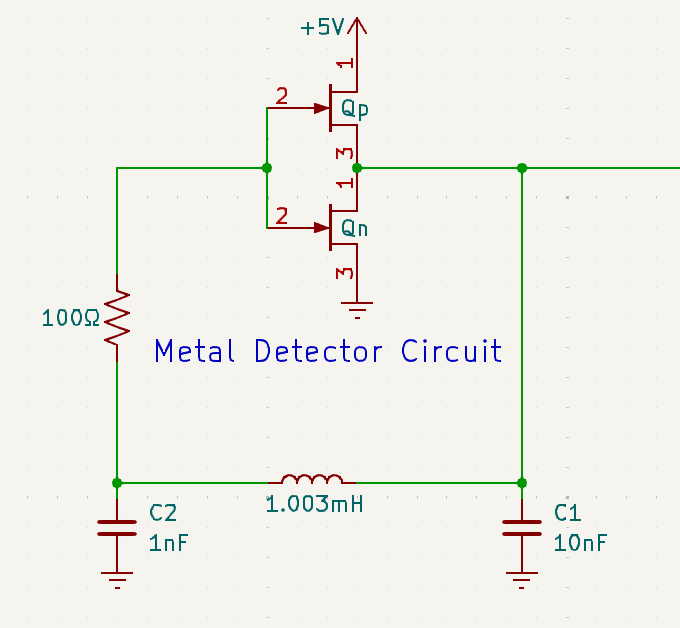
\includegraphics[width=0.5\textwidth]{Figures/metaldetector.png}
    \caption{Colpitts Oscillator with Discrete CMOS Inverter}
    \label{fig:metaldetector}
\end{figure}

\begin{figure}[htbp]
    \centering
    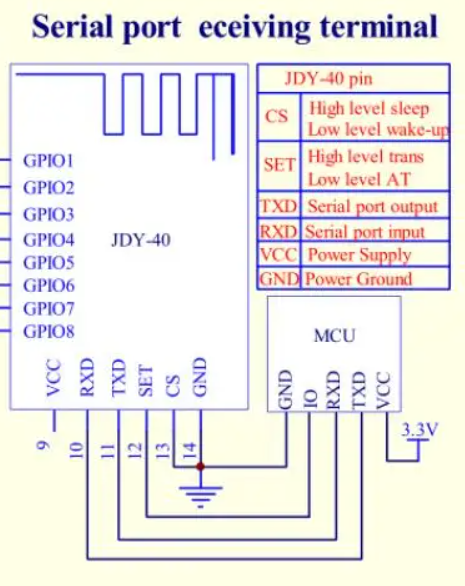
\includegraphics[width=0.5\textwidth]{Figures/jdy40.png}
    \caption{Example JDY-40 connections with a Microcontroller}
    \label{fig:JDY-40}
\end{figure}

\begin{figure}[htbp]
    \centering
    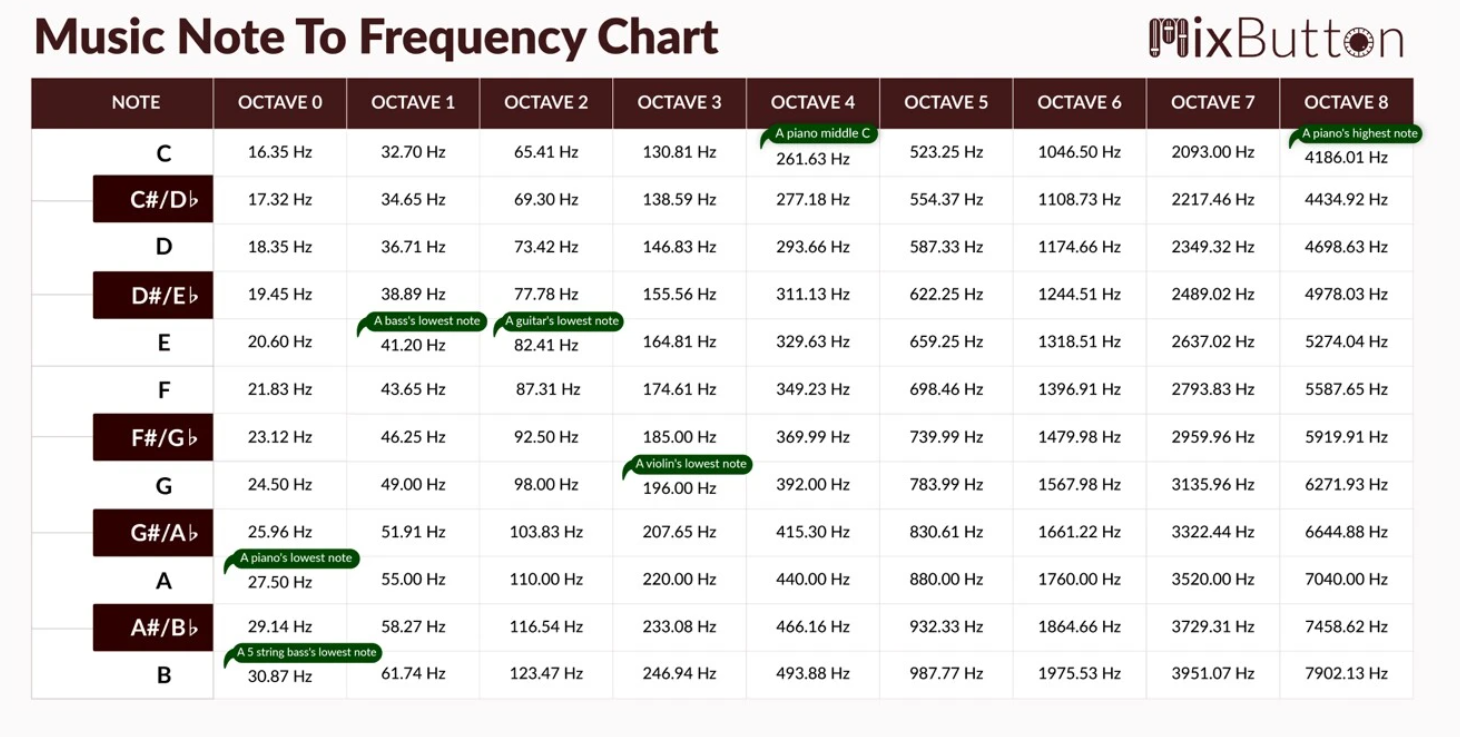
\includegraphics[width=0.8\textwidth]{Figures/Music_Frequencies.png}
    \caption{Musical Notes and their Frequencies}
    \label{fig:music_frequencies}
\end{figure}

\begin{table}[ht]
    \centering
    \begin{tabular}{@{}llll@{}}
        \toprule
        \textbf{Datetime}                & \textbf{Inductance X} & \textbf{Inductance Y} \\ \midrule
        2024-04-11 13:44:14.925344 & 487.0 & 480.0 \\
        2024-04-11 13:44:15.233376 & 483.0 & 487.0 \\
        2024-04-11 13:44:15.516551 & 461.0 & 483.0 \\
        2024-04-11 13:44:15.810678 & 435.0 & 461.0 \\
        2024-04-11 13:44:16.101832 & 418.0 & 435.0 \\ \addlinespace
        ...                            & ...   & ...   \\ \addlinespace
        2024-04-11 13:44:34.502735 & 490.0 & 490.0 \\
        2024-04-11 13:44:34.806378 & 490.0 & 490.0 \\
        2024-04-11 13:44:35.088966 & 492.0 & 490.0 \\
        2024-04-11 13:44:35.374161 & 490.0 & 490.0 \\
        2024-04-11 13:44:35.671002 & 490.0 & 490.0 \\ \bottomrule
    \end{tabular}
    \caption{Log Data : Inductance}
    \label{table:inductance_log_table}
\end{table}

\newpage
\begin{lstlisting} [language=C, caption={EFM8 : Timer 5 PWM Generation}, label={lst:efm8_timer5pwm}, basicstyle=\ttfamily\tiny]

if (count > 100)
    {
        count = 0;
    }
    if (PWM_percent_y >= 0)
    {
        LEFT_MOTOR_LHS = (count > left_wheel ) ? 0:1;
        RIGHT_MOTOR_LHS = (count > new_right_wheel) ? 0:1;
    }
    else
    {
        LEFT_MOTOR_LHS = (count > left_wheel) ? 1:0;
        RIGHT_MOTOR_LHS = (count > new_right_wheel) ? 1:0;
    }

    count++;

\end{lstlisting}

\begin{lstlisting} [language=C, caption={EFM8 : Timer 4 ISR}, label={lst:efm8_timer4isr}, basicstyle=\ttfamily\tiny]
    void Timer4_ISR (void) interrupt INTERRUPT_TIMER4 {
        int current_TR0 = TR0, current_TR5 = TR5;
        TR0 = 0, TR5 = 0;

        SFRPAGE=0x10;
        TF4H = 0; // Clear Timer4 interrupt flag
        TXcount++;

        if(TXcount >= 250){
            TXcount=0;
            flag == 0;
        }

        if (current_TR0 == 1) TR0 = 1;
        if (current_TR5 == 1) TR5 = 1;
    }
\end{lstlisting}

\begin{lstlisting} [language=C, caption={EFM8 : JDY-40 RX}, label={lst:efm8_jdy40rx}, basicstyle=\ttfamily\tiny]
void RX_XY() {
    if(RXU1()) {
	    getstr1(RXbuff);
	    clearUART1Buffer();
	    length = strlen(RXbuff);
        // printf("UNPARSED RX: %s\r\n", RXbuff);
	    if(length >= 12 && length <= 14){
	    	Trim(RXbuff, &commands[0],&commands[1], &commands[2]);
	    }
	}
}

void Trim(char *str, int *xin, int *yin, int *zyn) {
    int i, j;
    char * strStart = str;
    char *x = malloc(5 * sizeof(char));
    char *y = malloc(5 * sizeof(char));
    char *z = malloc(2 * sizeof(char));

    for (i = 0, j = 0; str[i] != '\0'; i++) {
        if (isdigit(str[i]) || str[i] == '-') {
            str[j++] = str[i];
        }
    }
    str[j] = '\0';  // Null-terminate the resulting string
    splitString(str, x, y, z);

    //printf("%p \n", y);
    //printf("%p \n", x);

    *xin = stringToInt(x);
    *yin = stringToInt(y);
    *zyn = stringToInt(z);


    free(x);
    free(y);
    free(z);
}
\end{lstlisting}

\begin{lstlisting} [language=C, caption={Frequency Calculation Function}, label={lst:frequencyfunction}, basicstyle=\ttfamily\tiny]
unsigned long GetFrequency_Hz(void) {
    long int count = GetPeriod(5);
    long int frequency = (SYSCLK*5.0)/(count*12);

    // printf("Frequency: %ld Hz\n", frequency);

    if (count>0) return frequency;
    else return 0;
}
\end{lstlisting}

\end{document}